\section{Introduction}
\label{sec:intro}

A verifier used as a training reward is a bit on each completion: accept or reject.
The usual summary of that bit is a rate, and Youden's $J = 1 - \mathrm{FPR} - \mathrm{FNR}$ folds the two rates into one number.
A moderate $J$ is often treated as good enough to train on, and there is evidence for that view.
\citet{rad2026rate} show that class-conditional noise with $J > 0$ rescales the time to learn and does not change the direction of a replicator flow.
\citet{plesner2026noise} find that symmetric noise up to 15 percent leaves peak validation accuracy close to clean training.
There is also evidence against it.
\citet{egashira2026delay} plant systematic verifier errors and find that the pattern of the error, not the rate or $J$, lines up with delay, plateau, or collapse.
Their arms were not calibrated to one rate, so pattern and rate moved together, and they ask for diagnostics that work without the oracle on every sample.
\citet{plesner2026noise} ask for noise that is fixed rather than redrawn, with the two rates varied separately.
This paper provides both: a design in which every error pattern has the same rate, and a step-0 diagnostic that is locked before training.

The running example is a phrase trigger.
One verifier accepts a wrong completion whenever it contains a fitted phrase.
A second accepts wrong completions at the same rate, chosen at random each time a completion is scored.
A third accepts wrong completions at the same rate when they contain a different phrase, one that is enriched among correct answers.
If only the rate mattered, the three would train alike.
A label that sorts errors into shared and random would call the first and third equally bad.
The claim tested here is sharper.
The random verifier stays close to a clean reward, and the two phrase verifiers, which are the same kind of rule at the same rate, can still end apart, because one phrase points toward correct answers and the other does not.

The argument is first-order, at the base policy.
Write the verifier as $V = O - \mathrm{FN} + \mathrm{FP}$.
The GRPO update at step 0 splits the same way.
Resampled noise, independent of the features given the oracle, multiplies the clean update by $J$ and adds no direction.
A fixed error adds the features it correlates with.
A held-out prompt moves only through the inner product of its features with the update, so an error that lives on one prompt stays there, and an error that rides a shared behaviour reaches prompts the trainer has not seen.
The scalar we lock before training, transfer precision, is the oracle accuracy of the outputs that the update favours.
It needs oracle labels on those favoured outputs and not on the whole pool: 192 labels per cell in the primary screen.

Pilot P0 makes this exact in finite worlds where the population update is known (Figure~\ref{fig:fates}).
On \texttt{hand\_noisy}, three verifiers share $J = \PZeroHandJ{}$ and end at held-out accuracy $\PZeroHandFpF{}$ for a shared exploit, $\PZeroHandFpI{}$ for a twin with the same base logits and no exploit coordinate, and $\PZeroHandNoise{}$ for noise resampled at the exploit's rates.
On \texttt{rf05}, at $J = \PZeroRfJ{}$, the same three end at $\PZeroRfFpF{}$, $\PZeroRfFpI{}$, and $\PZeroRfNoise{}$.
The shared exploit's transfer precision is $\PZeroHandTau{}$ and $\PZeroRfTau{}$.
On \texttt{hand\_clean}, the same shared rule has the same $J$, its transfer precision is $\PZeroCleanTau{}$, and it ends at $\PZeroCleanFpF{}$.
Shared structure is therefore not the same as harm, and the screen, unlike a structure label, tells the two cases apart.
On the grid used to choose the estimator, the Spearman correlation of the screen with trained accuracy is $\PZeroTauPoolRho{}$, against $\PZeroJRho{}$ for $J$.
One world is a documented failure: in a knife-edge world outside that grid, the screen is high and the long run still collapses (Section~\ref{sec:theory}).

\begin{figure*}[t]
\centering
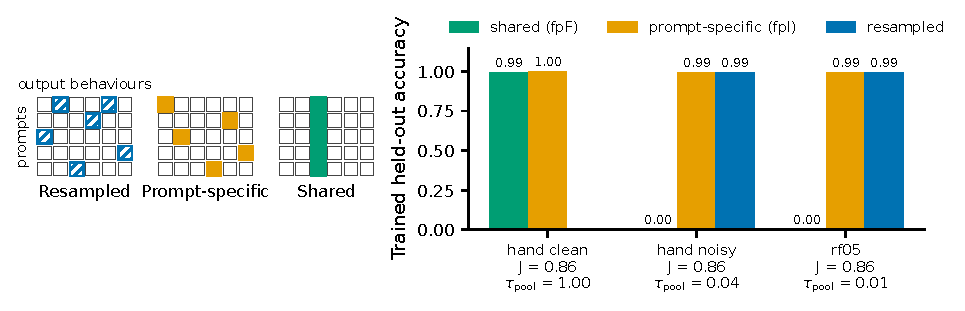
\includegraphics[width=\textwidth]{figures/fig1.pdf}
\caption{Left: three verifiers with one false-positive rate. Rows are prompts, columns are output behaviours, and a marked cell is an accepted wrong output. Resampled errors (hatched) are redrawn every time an output is scored. Prompt-specific errors are fixed, on a different behaviour in each prompt. A shared error is on the same behaviour in every prompt, so its update adds up across prompts and reaches held-out prompts. Right: trained held-out accuracy in pilot P0 for a shared exploit (\texttt{fpF}), a twin with the same base logits and no exploit coordinate (\texttt{fpI}), and noise resampled at the exploit's rates. The three worlds have the same $J$ to two decimals. Transfer precision separates the shared exploit that collapses from the one that does not.}
\label{fig:fates}
\end{figure*}

The study that tests this on language models is preregistered and split in two.
Stage A, on lab GPUs, is the discovery sample: five domains at Qwen3-1.7B with the full menu of arms, and the same five domains at Qwen3-4B.
Stage B is a prospective replication: the core menu at Qwen3-8B, 14B, and 32B, and math and code on OLMo-3-7B-SFT and Llama-3.1-8B-Instruct.
Each stage's confirmatory analysis is fixed now and computed once, when that stage is complete, and stage B's test uses only stage B's pairs.
The design is built so that a null result also answers a question.
Resampled controls say whether a fixed error differs from noise at its own rate.
Same-class pairs say whether the screen reads more than the structure label.
The baselines say whether the screen beats what a practitioner already has.

\paragraph{Contributions.}
\begin{itemize}
\item A decomposition of the step-0 GRPO update into the oracle direction and the two error directions, a transfer theorem for held-out prompts, and a screen that reads only the outputs the error direction favours (Theorem~\ref{thm:transfer}).
\item A matched-rate design in five domains. Shared and prompt-specific rules are calibrated to one false-positive rate and one false-negative rate, each with a resampled control. Two same-class pairs reverse only the direction the screen reads, so a rule that says ``shared errors are bad'' cannot pass them. Natural verifiers enter at their own measured rates.
\item A locked two-stage protocol. Forecasts, configuration, environment, and every input artefact are hashed before the first training step, and stage B replicates the screen from 8B to 32B and on two other families, on pairs stage A never sees.
\item The comparisons a practitioner would make. The screen is set against the error rate, $J$, gradient cosine, a probe, the pattern score of \citet{egashira2026delay}, a structure label, and a 25-step training run. The report also gives the oracle-label budget curve, the measured cost of the audit, and a patch chosen by the screen against a patch chosen by the error count.
\end{itemize}
% AFTER-RESULTS: (H3 and H10 hold) Add one sentence: the screen orders training outcomes at one rate, including inside one structure class.
% AFTER-RESULTS: (H3-replication holds) Add one sentence: the ordering replicates on models and families that stage A never used.
% AFTER-RESULTS: (H8 holds) The patch result is a use of the screen, not only a correlation.
% AFTER-RESULTS: (a headline test does not hold) State which one, and what the preregistered null means (Section~\ref{sec:study}).
